\documentclass{article} % For LaTeX2e
\usepackage{nips15submit_e,times}
\usepackage[colorlinks,linkcolor=red]{hyperref}
\usepackage{url}
\usepackage{amsmath}
\usepackage{graphicx}
\usepackage{float}
\usepackage{bm}
\usepackage{amssymb}
%\documentstyle[nips14submit_09,times,art10]{article} % For LaTeX 2.09


\title{CS499 Homework 9 (First Draft)}


\author{
	Intersteller\thanks{ Use footnote for providing further information
		about author (webpage, alternative address)---\emph{not} for acknowledging
		funding agencies.}
	Department of Computer Science
	Cranberry-Lemon University
	Pittsburgh, PA 15213
}

% The \author macro works with any number of authors. There are two commands
% used to separate the names and addresses of multiple authors: \And and \AND.
%
% Using \And between authors leaves it to \LaTeX{} to determine where to break
% the lines. Using \AND forces a linebreak at that point. So, if \LaTeX{}
% puts 3 of 4 authors names on the first line, and the last on the second
% line, try using \AND instead of \And before the third author name.

\newcommand{\fix}{\marginpar{FIX}}
\newcommand{\new}{\marginpar{NEW}}

\newtheorem{theorem}{}

%\nipsfinalcopy % Uncomment for camera-ready version

\begin{document}
	
	
	\maketitle
	
	
	\textbf{Exercise 9.1}\par
    We define$f_1:N\rightarrow N$\par
    $f_1\left(0\right)=0,
    f_1\left(1\right)=1,
    \cdots,
    f_1\left(n\right)=n.
    $\par
    We define $f_2:N\rightarrow N^2$ based on this graph:
    \begin{figure}[H]
  	\centering
  	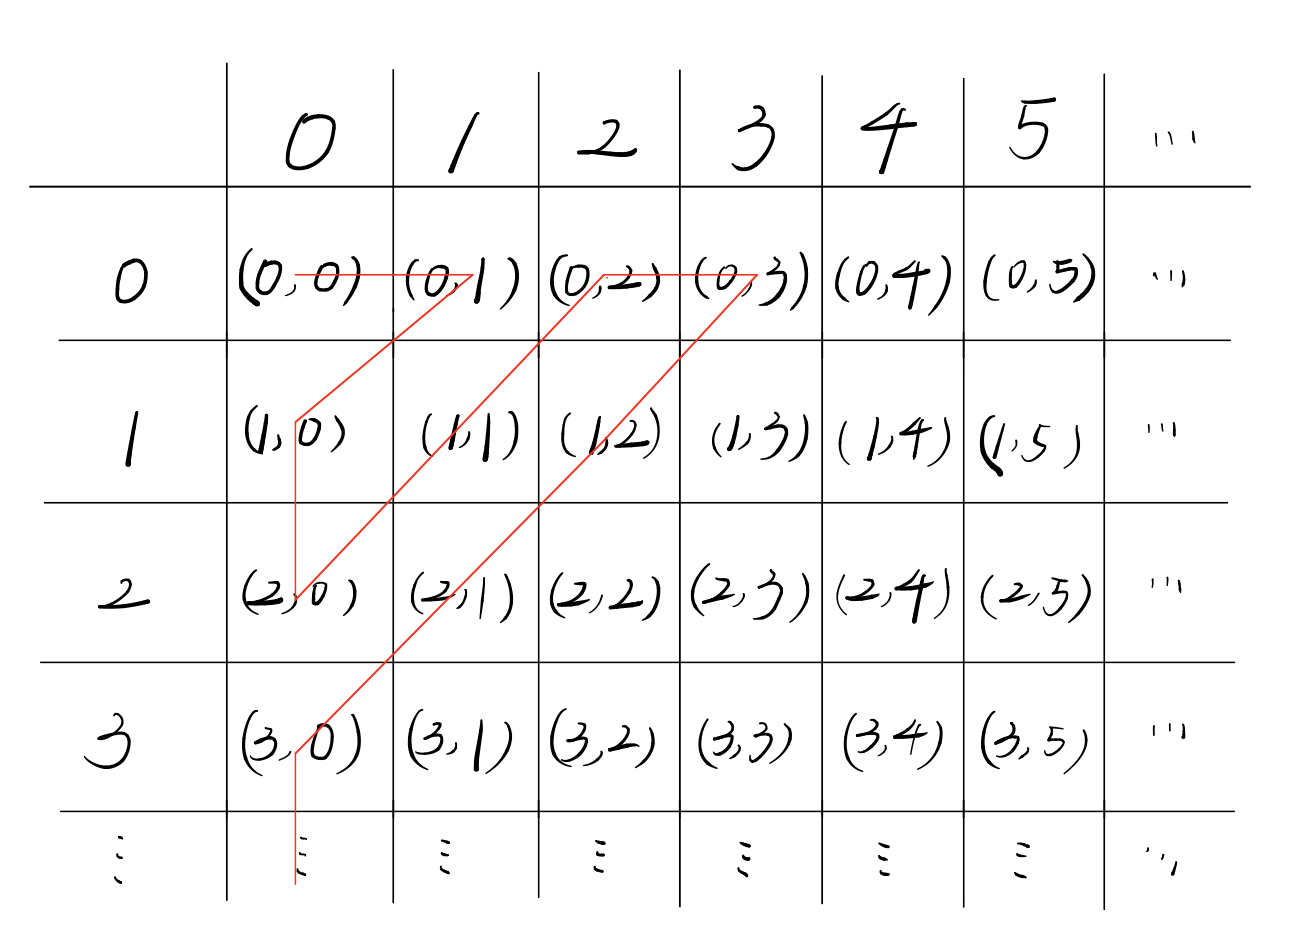
\includegraphics[width=8cm]{9_1_1.png}
  	\caption{}
  	\label{}
  	\end{figure}
    $f_2\left(0\right)=\left(0,0\right),f_2\left(1\right)=\left(0,1\right),f_2\left(2\right)=\left(1,0\right)\cdots$\par
    We define $f_3:N\rightarrow N^3$ based on this graph:
   \begin{figure}[H]
  	\centering
  	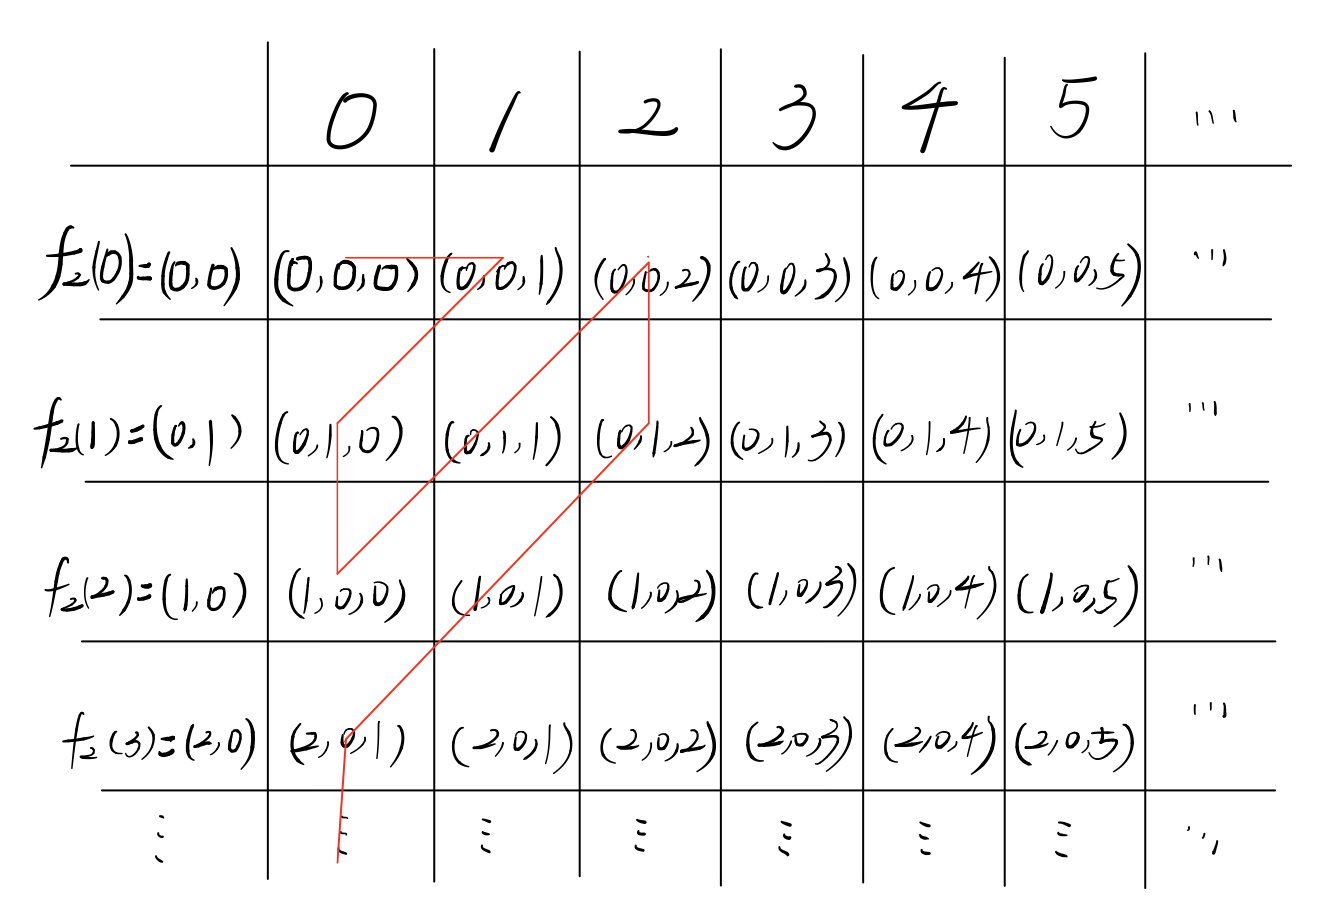
\includegraphics[width=8cm]{9_1_2.png}
  	\caption{}
  	\label{}
  	\end{figure}
    $f_2\left(0\right)=\left(0,0,0\right),f_2\left(1\right)=\left(0,0,1\right),f_2\left(2\right)=\left(0,1,0\right)\cdots$\par
    And so on, we can define $f_k,k\in N$.
    Now we can define a bijection $N\rightarrow N^*$ base on this graph:
    \begin{figure}[H]
  	\centering
  	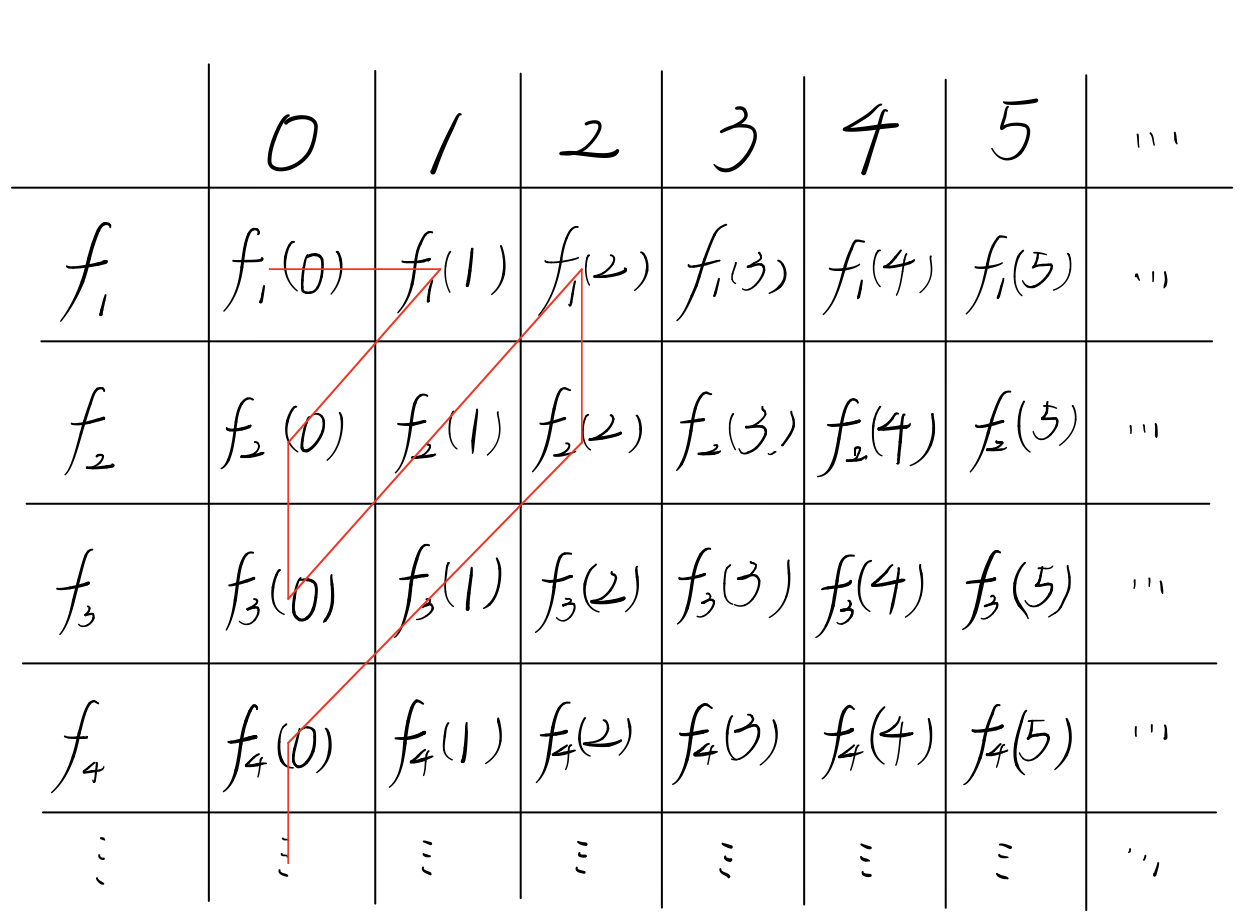
\includegraphics[width=8cm]{9_1_3.png}
  	\caption{}
  	\label{}
  	\end{figure}
    We have $0\rightarrow f_1\left(0\right),1\rightarrow f_1\left(1\right),2\rightarrow f_2\left(0\right)\cdots$. This is a bijection $N\rightarrow N^*$.


\textbf{Exercise 9.2}\par
We can define a bijection from $\{0,1\}^N$ to $\{0,1\}^N\times \{0,1\}^N$ as follows.\\
Given $A=(a_1a_2a_3a_4\cdots,b_1b_2b_3b_4\cdots)$, we define $f(A)=a_1b_1a_2b_2a_3b_3a_4b_4\cdots$. To be more precisely, 
$$ f(A)[i]=\left\{
\begin{aligned}
A[1][\frac{i+1}{2}],\ i\ is\ odd\ number \\
A[2][\frac{i}{2}],\ i\ is\ even\ number \\
\end{aligned}
\right.
$$
Obviously, for each $A\in \{0,1\}^N\times \{0,1\}^N$, there is only one $f(A)\in \{0,1\}^N$. For each $B\in \{0,1\}^N$, there is only one $B=f^{-1}(B)\in \{0,1\}^N\times \{0,1\}^N$. Therefore, $f$ is a bijection and $\{0,1\}^N\cong \{0,1\}^N\times\{0,1\}^N$.\\
Using the fact that $R\cong \{0,1\}^N$, we can get $R\cong R\times R$.

\textbf{Exercies 9.3}\par
We use the Cantor's method to proove that. For any $A\in (\{0,1\}^N)^N$, we define that $f(A)$ is the $\{0,1\}^N$ sequence we get by following the blue line as follows.
 
\begin{figure}[H]
    \centering
    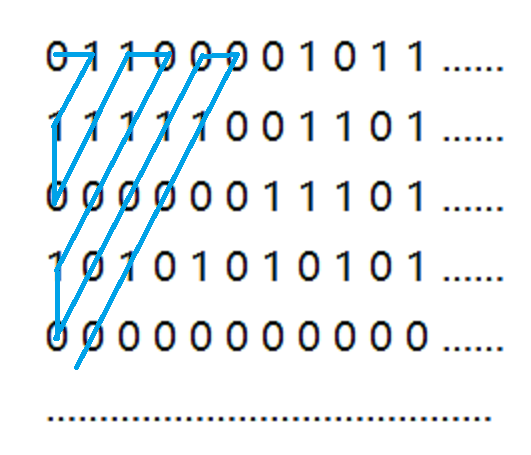
\includegraphics[width=8cm]{9_3_1.png}
    \caption{}
    \label{}
    \end{figure}
It is obvious that for any $B\in \{0,1\}^N$, we can get to $f^{-1}\in (\{0,1\}^N)^N$ by writing it down following the blue line. Therefore, $f$ is a bijection and $\{0,1\}\cong (\{0,1\}^N)^N$. Using the fact that $R\cong \{0,1\}^N$, we can get $R\cong R^N$.
	\textbf{Exercise 9.4}\par
	We know that one continuous function can be expressed by an infinite sequence of real numbers. 
	Thus we have   $\mathcal{F} \cong \mathbb{R}^{\mathbb{N}}$. According to \textbf{Exercise 9.3},  $\mathbb{R} \cong \mathbb{R}^{\mathbb{N}}$.
	So we have $\mathcal{F} \cong \mathbb{R}^{\mathbb{N}} \cong \mathbb{R}$.\par

	\textbf{Exercise 9.5}\par
    $000\cdots,100\cdots,1100\cdots,11100\cdots$ According to this rule, the first $n$ bits of the $n_{th}$ sequence are $1$, and the remaining bits are $0$. Obviously, these sequences constitute a countably and infinite chain.
	
	\textbf{Exercise 9.6}\par
	$100\cdots,0100\cdots,00100\cdots,000100\cdots$ According to this rule, the $n_{th}$ bit of the $n_{th}$ sequence is $1$, and the remaining bits are $0$. Obviously, these sequences constitute a countably and infinite antichain.
	\textbf{Exercise 9.7}\par
    	We can form a bijection $f$ from ${\{0,1\}}^{\mathbb{N}}$ to set $A$, which is a subset of ${\{0,1\}}^{\mathbb{N}}$ as follow:
	Assume a string $s$ is an element of ${\{0,1\}}^{\mathbb{N}}$ and $t=f(s)$, the $k$ digit of $s$ determines the $(2k-1)$-th to 
	$2k$-th digits of $t$ as the following rule:\par
	If $k$ digit of $s$ is $0$, then $(2k-1)$-th to $2k$-th digits of $t$ are $01$. If $k$ digit of $s$ is $1$, then $(2k-1)$-th to $2k$-th digits of $t$ are $10$. \par
	Here is an example :\par
	$$
	s=1011010........
	$$
	$$
	f(s)=10,01,10,10,01,10,01,......
	$$
	Obviously, $f$ is a bijection and $A$ is uncountable. Also, any two elements $t_{1},t_{2}$ of $A$ is not comparable since $01$ and $10$ can not be comparable.
	Thus $A$ is antichain required.\par
	\textbf{Exercise 9.8}\par
	 We can form a bijection $f$ from ${0,1}^N$ to set $A$, which is a subset of ${0,1}^N$ as follow: Assume a string $s$ is an element of ${0,1}^N$ and  $t=f(s)$, the first k digit of $s_1 ($we call it $s_k)$determines the $(2^{k}+1)-th$ to $2^{k+1}-th $ digits of $t ($ we  call them $t_{2^k+1} to t_{2^{k+1}}$ as the following rule:\par
	 
	 	 Consider the first k digits as a binary number $a_k$, then $t_{2^k+1}$ to $t_{2^k+a_k}$ are 1 and the $t_{2^k+a_k+1}$ to $t_{2^{k+1}}$ are 0. Specially, we define that the first 2 digits of t are always $'00'$.  
	 
	 Here is an example:
	 $$
	 s=1011......
	 $$
	 $$
	 f(s)=00,10,1100,11111000,1111111111100000,......
	 $$
	 Obviously, $f$ is a bijection and A is uncountable. Also, any two elements $t_1,t_2$ of A is comparable. Assume two elements $s_1,s_2$ is different and their first different digit is the k-th digit. The k-th element of $s_1$ is 1. Then for any $m$ such that $m \ge k$,the binary number of the first m digit of $s_1$ is greater than that of $s_2$, which leads to the conclusion that the according string of $t_1$ is "greater" than $t_2$. Thus A is the chain required. 
  \textbf{9.9}
	  For every sequence of $\{0,1\} ^N$, form a set$x_i={s_1,s_2,s_3,...}$ with all its prefixion as follow: assume that its first n digit is $a_1,a_2,...,a_n$,$s_n=\sum_{i=1}^N(a_i+1)\times 3^{i-1}$.Apparently every set $x_i$ is infinite and $x_i\in 2^N$. Call such bijection from a sequence of $\{0,1\}^N$ to a set $f$. Then we get a set $X=\{f(x)|x\in \{0,1\}^N\}$ which satisfy the demand. As $\{0,1\} ^N$ is uncountable, X is uncountable. And $f(x)$ is infinite. Whenever distinct $x,y \in X(x=\{s_{x1},s_{x2},...\})$, suppose $m=f^{-1}(x),n=f^{-1}(y)$ and assume the first different digit between m and n is the k-th digit. Then $x\cap y={s_{x1},s_{x2},...,s_{x(k-1)}}$, which is finite.
	 \textbf{question}
	 How to prove that $R$ is smaller than $2^R$.
	
\end{document}

